\chapter{Coniques}
\minitoc
\minilof
\minilot
\section{Définition monofocale et équation polaire}
Soient $F$ un point du plan, $\Dr$ une droite ne passant pas par $F$, $e$ un réel strictement positif.
\subsection{Définition monofocale}
\begin{defdef}
   On appelle conique de foyer $F$, de directrice $\Dr$ et d'excentricité $e$ l'ensemble des points $M$ du plan tels que
  \begin{equation}
    MF=e MH,
  \end{equation}
  où $H$ est le projeté orthogonal de $M$ sur $\Dr$.
\end{defdef}
\begin{defdef}
  On appelle axe focal de la conique $\con{e}$ la droite $\Delta$ perpendiculaire à la droite $\Dr$ passant par $F$.
\end{defdef}
\begin{prop}
  La conique $\con{e}$ est symétrique par rapport à l'axe focal $\Delta$.
\end{prop}
\begin{proof}
  On note $K$ le projeté orthogonal de $F$ sur $\Dr$ : $K=D \cap \Delta$. Soit $M \in \con{e}$ et $H$ son projeté orthogonal sur $\Dr$. Soit $M'$ le symétrique de $M$ par rapport à $\Delta$, $H'$ le projeté orthogonal de $M'$ sur $\Dr$ (c'est aussi le symétrique de $H$ par rapport à $\Delta$). Alors
\begin{equation}
  \frac{M'F}{M'H'} = \frac{MF}{MH} = e,
\end{equation}

donc le point $M'$ appartient à la conique $\con{e}$.
\end{proof}
Si on considère l'application $\fonction{\varphi}{P\setminus\{\Dr \cup F\}}{\Rplusetoile}{M}{\frac{MF}{MH}}$, où $H$ est le projeté orthogonal de $M$ sur $\Dr$, les coniques $\con{e}$ de directrice $\Dr$ sont les lignes de niveau de $\varphi$. On cherche les points d'intersection entre $\con{e}$ et l'axe $\Delta$. On note $K$ le projeté orthogonal de $F$ sur $\Dr$. On place l'origine des abscisses en $K$ et on oriente $\Delta$ de $K$ vers $F$, on note $d=KF$.

Soit M sur $\Delta$ le point d'abscisse $x$. Le projeté orthogonal de M sur la directrice $\Dr$ est le point K, puisque $\Dr$ et $\Delta$ sont orthogonal et se croisent en K. On a alors la suite d'équivalence suivante~:
\begin{align}
  M \in \con{e} &\iff MF = e MK \\
  &\iff MF^2=e^2 MK^2 \\
  &\iff (x-d)^2=e^2 x^2\\
  &\iff x^2+d^2-2xd=e^2 x^2\\
  &\iff x^2(1-e^2)-2xd+d^2=0.
\end{align}
On distingue deux cas~:
\begin{itemize}
\item si $e=1$, alors le point M est sur la conique si et seulement si $x=\frac{d}{2}$. Il y a donc un unique point d'intersection entre la conique $\con{1}$ est son axe focal $\Delta$, c'est le milieu de $[KF]$. Cette conique est une parabole;
\item sinon comme $1-e^2 \neq 0$, on peut calculer le discriminant de ce trinôme qui vaut $(2de)^2$, alors les deux racines réelles du trinôme sont $x_1=\frac{d}{1+e}$ et $x_2=\frac{d}{1-e}$. Soient les points d'intersections $A_1$ et $A_2$ de $\con{e}$ et $\Delta$, d'abscisse respectives $x_1$ et $x_2$. Alors $\vect{KA}=\frac{1}{1+e} \vect{KF}$ et $\vect{KA'}=\frac{1}{1-e} \vect{KF}$. On peut distinguer deux sous-cas~:
  \begin{itemize}
  \item si $e<1$ alors $x_1$ et $x_2$ sont positifs et les deux points $A$ et $A'$ sont du même côté de $\Dr$ que $F$. On dira que $\con{e}$ est une ellipse;
  \item si $e>1$ alors $A$ est du même côté que $F$ mais $A'$ est de l'autre, dans ce cas là on dira que $\con{e}$ est une hyperbole.
  \end{itemize}
\end{itemize}

\subsection{Équation polaire de $\con{e}$}
On munit le plan de la base orthonormale $(\vi,\vj)$ où $\vi=\frac{\vect{FK}}{\norme{\vect{FK}}}$ et où $\vj$ est tel que $(\vi,\vj)=\frac{\pi}{2}$ et $\norme{\vj}=1$. On se place dans le repère $\Rep=(F,\vi,\vj)$. Notons $d=FK$, une équation de $\Dr$ dans $\Rep$ est $x=d$ et son équation polaire dans $\Rep$ est $\rho=\frac{d}{\cos \theta}$. Soient un point $M$ du plan et son système de coordonnées polaires $(\rho,\theta)$ : $\vect{FM}=\rho\vect{u}_\theta$, alors~:
\begin{align}
  M \in \con{e} &\iff MF = e MH \\
  &\iff \abs{\rho}=e\abs{d-\rho \cos\theta}\\
  &\iff \begin{cases}\rho = ed-e\rho\cos\theta \\ \text{ou}\\ \rho = e\rho\cos\theta-ed \end{cases} \\
  &\iff  \begin{cases}\rho = \frac{ed}{1+e\cos\theta} \\ \text{ou}\\ \rho = \frac{-ed}{1-e\cos\theta} \end{cases}.
\end{align}
On obtient deux équations polaires, mais ces deux équations sont les mêmes~: en effet, si $(\rho,\theta)$ est un s.c.p.\ de $M$ alors $\rho=\frac{ed}{1+e\cos\theta}$ et donc en prenant l'opposé $-\rho=\frac{-ed}{1-e\cos(\theta+\pi)}$ et donc $(-\rho,\theta+\pi)$, étant un deuxième s.c.p.\ de $M$ dans $\Rep$ vérifie la deuxième équation. Alors~:
\begin{equation}
  M(\rho,\theta) \in \con{e} \iff \rho=\frac{ed}{1+e\cos\theta}.
\end{equation}
$\rho=\frac{ed}{1+e\cos\theta}$ est une équation polaire de la conique $\con{e}$.
\begin{enumerate}
\item Si on oriente la droite (FK) dans l'autre sens on obtient une équation du même type avec un signe négatif;
\item l'équation est la même pour toutes les valeurs de l'excentricité, mais le domaine dans lequel varie $\theta$ dépend de l'excentricité.
\end{enumerate}

\section{Équations réduites}
\label{sec:eqred}
Soit $\con{e}$ la conique de foyer $F$, de directrice $\Dr$, d'excentricité $e$. On note $d=d(F,\Dr)>0$. On pose $p=ed$, $p$ est appelé le paramètre de la conique $\con{e}$. On se place dans le ROND $(F,\vi,\vj)$ avec $\vi=\frac{\vect{KF}}{KF}$. Dans ce repère, $F(0,0), K(-d,0)$ et soit $M(x,y)$ un point du plan, $H$ le projeté orthogonal de $M$ sur $\Dr$, $H(-d,y)$. Alors~:
\begin{align}
  M \in \con{e} &\iff MF = e MH \\
  &\iff MF^2 = e^2 MH^2\\
  &\iff x^2+y^2=e^2(x+d)^2.
\end{align}

\subsection{Cas de la parabole}
Soit $S$ l'unique point d'intersection entre $\con{1}$ et $\Delta$. Le point $S$ est le sommet de la parabole, c'est aussi le milieu de $[KF]$, alors $S\left(\frac{-d}{2}\right)$. On adopte un nouveau repère~: le ROND $(S,\vi,\vj)$, si $M$ a pour coordonnées $(x,y)$ dans $(F,\vi,\vj)$ et $(X,Y)$ dans $(S,\vi,\vj)$ alors $X=x+\frac{d}{2}$ et $Y=y$. Ainsi~:
\begin{align}
  M(X,Y) \in \con{1} &\iff \left(X-\frac{d}{2}\right)^2+Y^2=\left(X+\frac{d}{2}\right)^2\\
  &\iff \left(X-\frac{d}{2}\right)^2 - \left(X+\frac{d}{2}\right)^2+Y^2=0\\
  &\iff Y^2=2dX=2pX,
\end{align}
puisque $p=ed=d$.
\begin{theo}
Soit $\P$ une parabole de foyer $F$ de directrice $\Dr$. Il existe un repère orthonormal $(S,\vi,\vj)$ dans lequel $\P$ a pour équation $Y^2=2pX$, c'est ce qu'on appelle l'équation réduite de la parabole $\P$.

Réciproquement, si $p$ est un réel strictement positif, l'ensemble des points représentés par l'équation cartésienne $Y^2=2pX$ dans un repère orthonormal $\rond$ est une parabole de foyer $F\left(\frac{p}{2},0\right)$, de directrice $\Dr$ et d'équation $X=\frac{-p}{2}$. Le nombre $p$ est le paramètre de la parabole. Un paramétrage de la parabole est~:
  \begin{equation}
    \forall t \in \R \quad
    \begin{cases}
      x(t)=\frac{t^2}{2p} \\
      y(t)=t
    \end{cases}.
  \end{equation}
\end{theo}

Une parabole est représentée sur la figure~\ref{fig:parabole}.

\begin{figure}[!h]
  \centering
  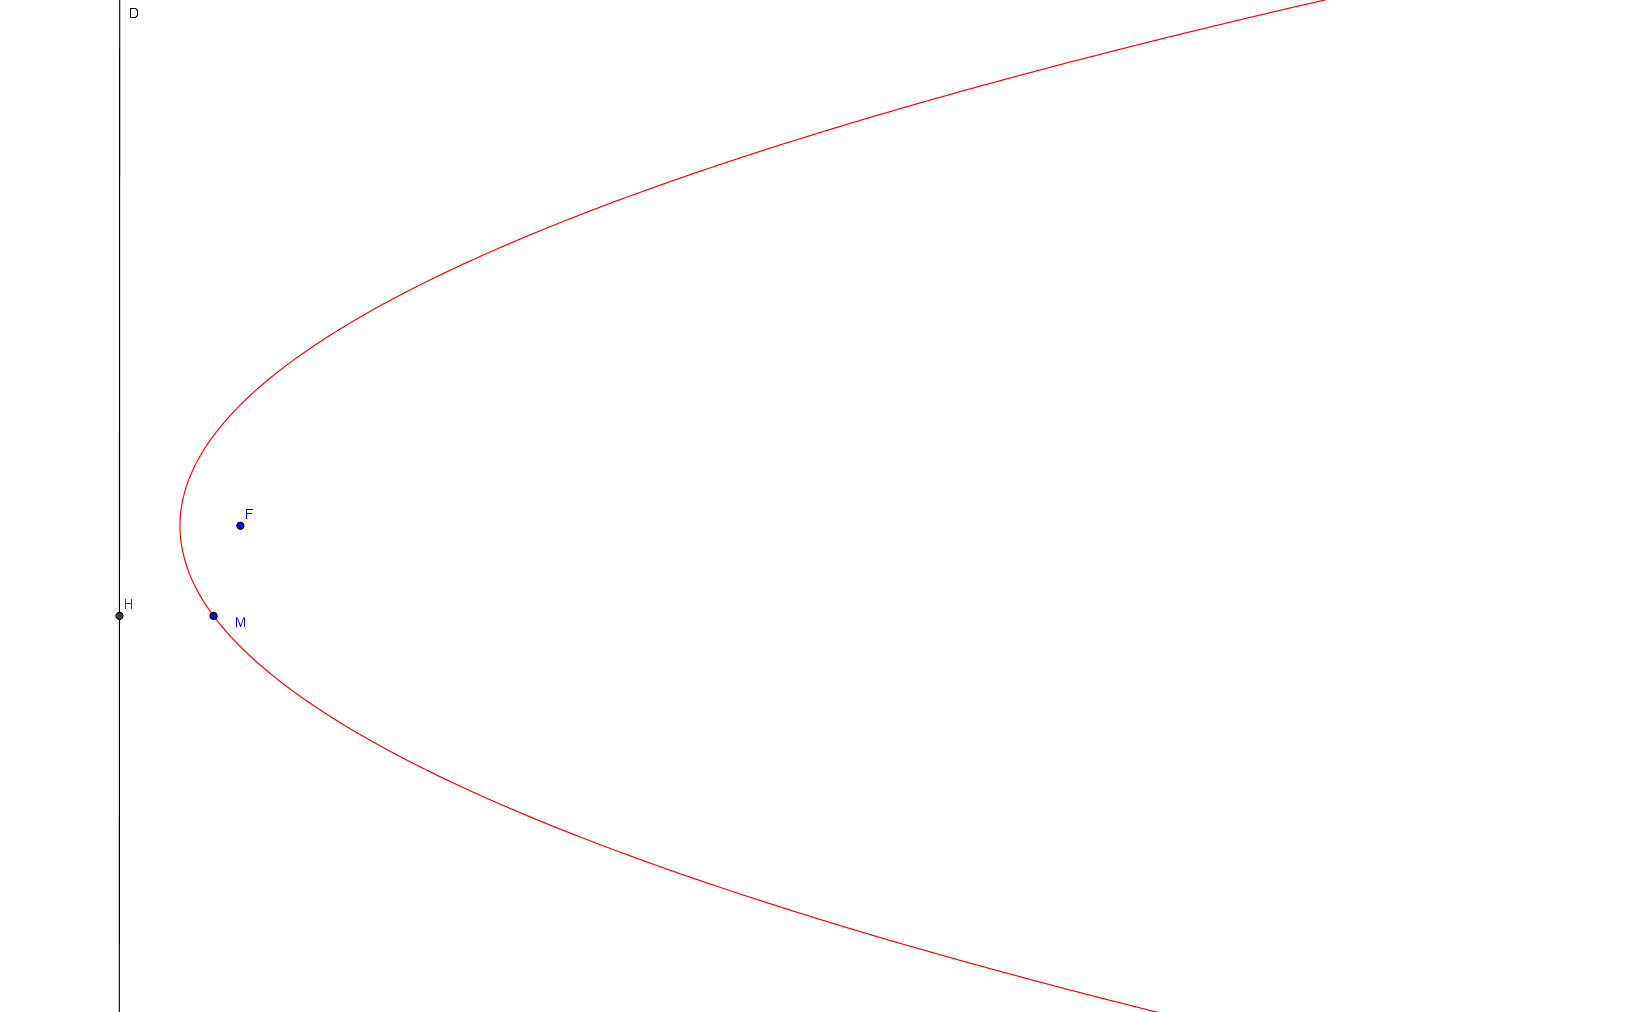
\includegraphics[width=\textwidth, scale=1]{parabole.png}
  \caption{Représentation graphique d'une parabole}
  \label{fig:parabole}
\end{figure}


\subsection{Cas des coniques à centre ($e\neq 1$)}
Dans ce cas la conique $\con{e}$ est son axe focal $\Delta$ on deux points d'intersection. Dans le repère $(K,\vi,\vj)$, ce sont les points $A(\frac{d}{1+e},0)$ et $A'(\frac{d}{1-e},0)$. Ces deux points sont les sommets de la conique $\con{e}$. On définit le milieu O de [AA'] et on se place dans le repère orthonormal $\rond$. Alors $\vect{KO}=\frac{1}{2}\left(\frac{d}{1+e}+\frac{d}{1-e}\right)\vi=\frac{d}{1-e^2}\vi$. Si M a pour coordonnées (x,y) dans $(K,\vi,\vj)$ et (X,Y) dans $\rond$ alors puisque $\vect{OM}=\vect{OK}+\vect{KM}=\vect{KM}-\frac{d}{1-e^2}\vi$ donc $X=x-\frac{d}{1-e^2}$ et $Y=y$. Alors on peut noter les coordonnées dans le nouveau repère~:
\begin{equation}
  K\left(-\frac{d}{1-e^2},0\right) \ F\left(-\frac{de^2}{1-e^2},0\right) \ A\left(-\frac{de}{1-e^2},0\right) \ A'\left(\frac{de}{1-e^2},0\right)
\end{equation}
Soit un point $M(x,y)$ et son projeté sur la directrice $H\left(-\frac{d}{1-e^2},Y\right)$. Alors~:
\begin{align}
  M \in \con{e} &\iff MF^2=e^2 MH^2\\
  &\iff \left(X+\frac{de^2}{1-e^2}\right)^2+Y^2=e^2 \left(X+\frac{d}{1-e^2}\right)^2\\
  &\iff X^2+\left(\frac{de^2}{1-e^2}\right)^2+Y^2=e^2 X^2+e^2\left(\frac{d}{1-e^2}\right)^2\\
&\iff X^2(1-e^2)+Y^2=\frac{d^2e^2}{1-e^2}=\frac{p^2}{1-e^2}.
\end{align}
Alors finalement, on distingue deux sous-cas.

\subsubsection{Cas des hyperboles ($e>1$)}
Si on pose $a=\frac{p}{e^2-1}$ et $b=\frac{p}{\sqrt{e^2-1}}$, alors dans le repère $\rond$ l'équation devient~:
\begin{equation}
  M(X,Y) \in \con{e} \iff \frac{X^2}{a^2}-\frac{Y^2}{b^2}=1
\end{equation}
\begin{theo}
  Il existe une repère orthonormal direct dans lequel l'hyperbole admet pour équation cartésienne~:
  \begin{equation}
    \frac{X^2}{a^2}-\frac{Y^2}{b^2}=1,
  \end{equation}
avec $a$ et $b$ des réels strictement positifs
\end{theo}
\begin{prop}
  \begin{enumerate}
  \item $p=\frac{b^2}{a}$ et $e^2-1=\frac{b^2}{a^2}$;
  \item si on pose $c=\sqrt{a^2+b^2}$, alors $e=\frac{c}{a} \ d=\frac{b^2}{c}$;
  \item le foyer F a pour coordonnées $(c,0)$ et la directrice $\Dr$ a pour équation $X=\frac{a^2}{c}$
  \end{enumerate}
\end{prop}
\begin{proof}
  \begin{enumerate}
  \item $\frac{b^2}{a}=\frac{\frac{p^2}{e^2-1}}{\frac{p}{e^2-1}}=p$ et $\frac{b^2}{a}=\frac{\frac{p^2}{e^2-1}}{\frac{p^2}{(e^2-1)^2}}=e^2-1$;
  \item $c=\sqrt{1+\left(\frac{b}{a}\right)^2}=\sqrt{1+e^2-1}=e$ puisque $e>0$ et $d=\frac{p}{e}=\frac{b^2}{a} \frac{a}{c}=\frac{b^2}{c}$;
  \item à la base l'abscisse de F est $-\frac{de^2}{1-e^2}=\frac{-pe}{1-e^2}=ae=c$ et l'équation de la courbe est $X=-\frac{d}{1-e^2}=-\frac{p/e}{1-e^2}=\frac{a}{e}=\frac{a^2}{c}$
  \end{enumerate}
\end{proof}
\begin{theo}[Théorème réciproque]
  Soient deux réels strictement positifs $a$ et $b$ et $c=\sqrt{a^2+b^2}$, un repère orthonormal $R=\rond$. La courbe d'équation cartésienne dans $R$ $\frac{X^2}{a^2}-\frac{Y^2}{b^2}=1$ est une hyperbole de foyer $F(-c,0)$ et de directrice $\Dr$ d'équation $X=\frac{a^2}{c}$ d'excentricité $e=\frac{c}{a}$ et de paramètre $p=\frac{b^2}{a}$.
\end{theo}
L'hyperbole $\H$ est aussi l'hyperbole de foyer $F'(-c,0)$ de directrice $\Dr ':X=-\frac{a^2}{c}$. Les intersections de $\H$ avec l'axe focal sont appelés les sommets de l'hyperbole. Ce sont les points $A(a,0)$ et $A'(-a,0)$.
\begin{prop}
  L'hyperbole $\H$ est la réunion des deux courbes paramétrées suivantes~:
  \begin{equation}
    \Gamma_1 : x(t)=a\cosh(t), y(t)=b\sinh(t) \quad \Gamma_2 : x(t)=-a\cosh(t), y(t)=b\sinh(t)
  \end{equation}
\end{prop}
\begin{proof}
  \begin{itemize}
  \item On démontre dans ce premier point l'inclusion $\Gamma_1 \subset \H$~: Soit un point $M(t)(x(t),y(t)) \in \Gamma_1$ alors pour chaque instant $t \in \R$, $\frac{x(t)^2}{a^2}-\frac{y(t)^2}{b^2}=\cosh^2(t)-\sinh^2(t)=1$ donc le point $M(t)$ est sur l'hyperbole.
  \item On démontre de la même manière l'inclusion  $\Gamma_2 \subset \H$
  \item Démontrons maintenant l'inclusion inverse $\H \in \Gamma_1\cup\Gamma_2$. Soit un point $M(x,y)$ sur l'hyperbole, on pose $t=\argsh\left(\frac{y}{b}\right)$ alors $y=b\sinh(t)$ et puisque le point est sur l'hyperbole on écrit~: $\frac{x^2}{a^2}=1+\frac{y^2}{b^2}=\cosh(t)$ donc $x^2=(a\cosh(t))^2$. Si $x\geq 0$ alors $x=a\cosh(t)$ et le point M est sur $\Gamma_1$ sinon $x=-a\cosh(t)$ et il est sur $\Gamma_2$. Dans tous les cas le point M est dans l'union $\Gamma_1 \cup \Gamma_2$.
  \end{itemize}
Finalement $\H=\Gamma_1 \cup \Gamma_2$.
\end{proof}
\begin{prop}
  L'hyperbole $\H$ admet pour asymptote les droites d'équations $y\frac{b}{a}x$ et $y\frac{-b}{a}x$.
\end{prop}
\begin{proof}
  Étudions la courbe paramétrée $\Gamma_1$~: lorsque $t \to +\infty$ alors $x$ et $y$ deviennent infinis, il y a donc une branche infinie. Le rapport $\frac{y(t)}{x(t)}=\frac{b}{a} \tanh(t)$ tend vers $\frac{b}{a}$. Ainsi la courbe admet une direction asymptotique de pente $\frac{b}{a}$ et la différence $y(t) -\frac{b}{a}x(t)=b(\sinh t -\cosh t)=-b\e^{-t}$ tend vers 0. Alors la courbe admet bien la droite d'équation $y=\frac{b}{a}x$ pour asymptote. On raisonne de la même manière en $t\to -\infty$ et pour la courbe $\Gamma_2$.
\end{proof}
Si $a=b$, on dit que l'hyperbole est équilatère et les asymptotes sont les bissectrices.


\subsubsection{Cas des ellipses ($e<1$)}
Si on pose $a=\frac{-p}{1-e^2}$ et $b=\frac{p}{\sqrt{1-e^2}}$, alors dans le repère $\rond$ l'équation devient~:
\begin{equation}
  M(X,Y) \in \con{e} \iff \frac{X^2}{a^2}+\frac{Y^2}{b^2}=1
\end{equation}
\begin{theo}
  Il existe une repère orthonormal direct dans lequel l'ellipse admet pour équation cartésienne~:
  \begin{equation}
    \frac{X^2}{a^2}+\frac{Y^2}{b^2}=1
  \end{equation}
  avec $a$ et $b$ des réels strictement positifs.
\end{theo}
\begin{prop}
  \begin{enumerate}
  \item $p=\frac{b^2}{a}$ et $1-e^2=\frac{b^2}{a^2}$;
  \item si on pose $c=\sqrt{a^2-b^2}$, alors $e=\frac{c}{a}$ et $d=\frac{b^2}{c}$;
  \item le foyer F a pour coordonnées $(c,0)$ et la directrice $\Dr$ a pour équation $X=\frac{a^2}{c}$
  \end{enumerate}
\end{prop}
\begin{proof}
  \begin{enumerate}
  \item $\frac{b^2}{a}=\frac{\frac{p^2}{1-e^2}}{\frac{p}{1-e^2}}=p$ et $\frac{b^2}{a^2}=\frac{\frac{p^2}{1-e^2}}{\frac{p^2}{(1-e^2)^2}}=1-e^2$;
  \item $\frac{c}{a}=\sqrt{1-\left(\frac{b}{a}\right)^2}=\sqrt{1-1+e^2}=e$ puisque $e>0$ et $d=\frac{p}{e}=\frac{b^2}{a} \frac{a}{c}=\frac{b^2}{c}$;
  \item à la base l'abscisse de $F$ est $-\frac{de^2}{1-e^2}=\frac{-pe}{1-e^2}=ae=c$ et l'équation de la courbe est $X=-\frac{d}{1-e^2}=-\frac{p/e}{1-e^2}=\frac{a}{e}=\frac{a^2}{c}$
  \end{enumerate}
\end{proof}
\begin{theo}[Théorème réciproque]
  Soient deux réels strictement positifs $a$ et $b$ et $c=\sqrt{a^2-b^2}$, un repère orthonormal $R=\rond$. La courbe d'équation cartésienne dans $R$ $\frac{X^2}{a^2}+\frac{Y^2}{b^2}=1$ est une ellipse de foyer $F(c,0)$ et de directrice $\Dr$ d'équation $X=\frac{a^2}{c}$ d'excentricité $e=\frac{c}{a}$ et de paramètre $p=\frac{b^2}{a}$.
\end{theo}
%L'ellipse $\Elli$ est aussi l' de foyer $F'(-c,0)$ de directrice $\Dr ':X=-\frac{a^2}{c}$. Les intersections de $\H$ avec l'axe focal sont appelés les sommets de l'hyperbole. Ce sont les points $A(a,0)$ et $A'(-a,0)$.
\begin{prop}
  L'ellipse $\Ell$ est la courbe paramétrée suivante~:
  \begin{equation}
    \Gamma : x(t)=a\cos(t), y(t)=b\sin(t).
  \end{equation}
\end{prop}
% \begin{proof}
%   %% À faire
% \end{proof}


\section{Définition bifocale des coniques à centre}
\subsection{Définition bifocale de l'ellipse}
\begin{prop}
  \label{prop:bifellipse}
  Soient $F$ et $F'$ deux points distincts et $a$ un réel tel que $2a>FF'$. Alors l'ensemble des points M du plan tel que $MF+MF'=2a$ est une ellipse de foyers $F$ et $F'$.
\end{prop}
\begin{proof}
  Soit O le milieu de $[FF']$ et le vecteur $\vi=\frac{\vect{FF'}}{FF'}$ et le vecteur $\vj$ tel que le repère $R=\rond$ soit orthonormal direct. Les coordonnées de F et F' sont tels que $F'(c,0)$ et $F(-c,0)$. Soit $\epsilon=\enstq{M \in \P}{MF+MF'=2a}$, pour tout point $M(x,y)$,
  \begin{align}
    M \in \epsilon & \iff MF+MF'=2a \\
    & \iff \sqrt{(x+c)^2+y^2} + \sqrt{(x-c)^2+y^2}=2a \\
    & \iff (x+c)^2+y^2+(x-c)^2+y^2 \notag \\
    & \phantom{\iff} + 2\sqrt{((x+c)^2+y^2)((x-c)^2+y^2)}=4a^2 \label{eq:tag:1}\\
    & \iff x^2+c^2+y^2+\sqrt{(x^2+c^2+y^2)^2-4c^2x^2}=2a^2\\
    & \iff \begin{cases} (x^2+c^2+y^2)^2-4c^2x^2 = (2a^2-(c^2+y^2+x^2))^2 \\ x^2+y^2 \leq 2a^2 -c^2\\\end{cases}\\
    & \iff \begin{cases} (x^2+c^2+y^2 + 2a^2-(c^2+y^2+x^2)) \\ \times (x^2+c^2+y^2 - 2a^2+(c^2+y^2+x^2))=4c^2x^2  \\ x^2+y^2 \leq 2a^2 -c^2\end{cases}\\
    & \iff \begin{cases} 2a^2(2x^2+2y^2+2c^2-2a^2)=4c^2x^2  \\ x^2+y^2 \leq 2a^2 -c^2\end{cases}\\
    & \iff \begin{cases} (a^2-c^2)x^2 +a^2y^2=(a^2-c^2)a^2  \\ x^2+y^2 \leq 2a^2 -c^2\end{cases}
  \end{align}
L'équation~\eqref{eq:tag:1} est justifiée puisque les deux membres sont positifs. Si on  pose $b=\sqrt{a^2-c^2}$, $2a>FF'=2c$ donc $a>c>0$, alors
\begin{align}
  M \in \epsilon & \iff \begin{cases} b^2x^2 +a^2y^2=b^2a^2 \\ x^2+y^2 \leq a^2 +b^2\\\end{cases}\\
  & \iff \begin{cases} \frac{x^2}{a^2} +\frac{y^2}{b^2}=1\\ x^2+y^2 \leq a^2 +b^2 \\\end{cases}
\end{align}
Si le couple $(x,y)$ vérifie la première équation du système alors $\frac{x^2}{a^2}=1-\frac{y^2}{b^2}\leq 1$ et $\frac{y^2}{b^2}=1-\frac{x^2}{a^2} \leq 1$ donc $x^2 \leq a^2$ et $y^2 \leq b^2$ et donc $x^2+y^2 \leq a^2+b^2$ ce qui correspond à la deuxième équation du système.
Alors $M \in \epsilon \iff \frac{x^2}{a^2} +\frac{y^2}{b^2}=1$ donc $\epsilon$ est une ellipse et $c=\sqrt{a^2-b^2}>0$, $\epsilon$ est une ellipse de foyer F et F'.
\end{proof}
Soit $\fonction{f}{\P}{\R}{M}{MF+MF'}$, un réel $c$ tel que $2c=FF'$, $\lambda>c$ et l'ensemble $X_\lambda=\enstq{M \in \P}{f(M)=\lambda}$ avec pour tout point M du plan $FF'\leq MF+MF'$.
\begin{itemize}
\item Si $\lambda < FF'$ alors $X_\lambda=\emptyset$;
\item sinon si $\lambda=FF'$ alors $FF'=MF+MF'$ si et seulement si $M \in [F,F']$ soit si et seulement si $X_\lambda=[FF']$;
\item sinon si $\lambda >FF'$ alors $X_\lambda$ est une ellipse de foyer $F$ et $F'$.
\end{itemize}

On a représenté une ellipse sur la figure~\ref{fig:ellipse}.

\begin{figure}[!h]
  \centering
  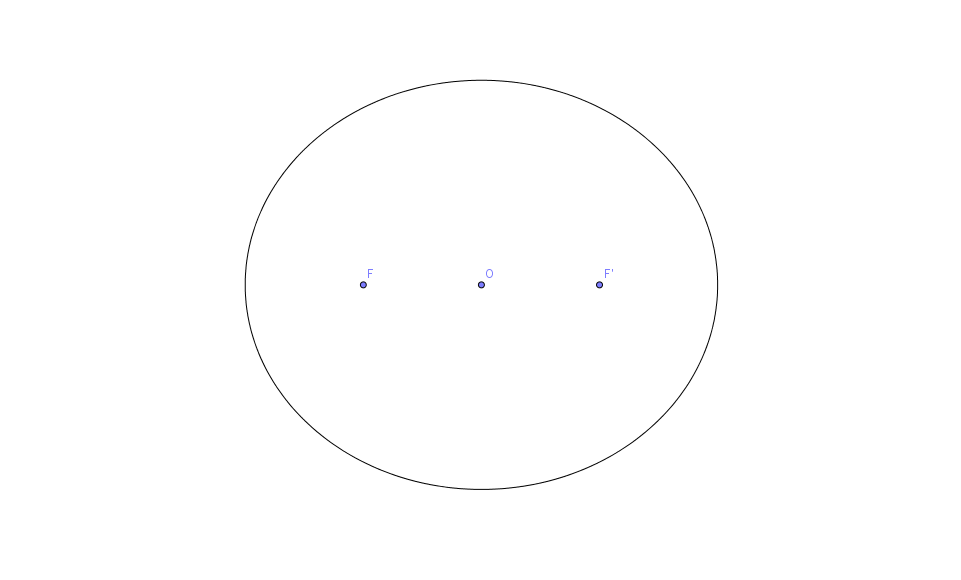
\includegraphics[width=\textwidth]{./ellipse.png}
  \caption{Représentation d'une ellipse}
  \label{fig:ellipse}
\end{figure}


\subsection{Définition bifocale de l'hyperbole}
\begin{prop}
  Soient $F$ et $F'$ deux points distincts. Soit $a$ un réel tel que $0<2a<FF'$. L'ensemble $\H$ des points M du plan tels que $\abs{MF-MF'}=2a$ est une hyperbole de foyer F et F'.
\end{prop}
\begin{proof}
  On se place dans le même repère que pour la démonstration de~\ref{prop:bifellipse}. On note $F(-c,0)$ et $F'(c,0)$. Pour tout point $M(x,y)$  on a~:
  \begin{align}
    M \in \H & \iff \abs{MF'-MF}=2a \\
    & \iff \abs{\sqrt{(x+c)^2+y^2}-\sqrt{(x-c)^2+y^2}}=2a \\
    & \iff (x+c)^2 +y^2 + (x-c)^2 + y^2 \notag \\ & \phantom{\iff} -2\sqrt{[(x-c)^2+y^2][(x+c)^2+y^2]}=4a^2\\
    & \iff 2x^2+2y^2+2c^2-4a^2=2\sqrt{[(x-c)^2+y^2][(x+c)^2+y^2]}\\
    & \iff \begin{cases}(x^2+y^2+c^2-2a^2)^2=(x^2+y^2+c^2)^2-4c^2x^2 \\ x^2+y^2+c^2-2a^2 \geq 0\end{cases}\\
    & \iff \begin{cases}-a^2(x^2+y^2+c^2-a^2)+c^2x^2=0 \\ x^2+y^2+c^2-2a^2 \geq 0\end{cases}\\
    & \iff \begin{cases}(c^2-a^2)x^2 - a^2y^2=a^2(c^2-a^2) \\ x^2+y^2 \geq 2a^2-c^2\end{cases}.
  \end{align}
  Or $0<2a<FF'=2c$ donc $0<a<c$ et on pose $b=\sqrt{c^2-a^2}$, alors
  \begin{equation}
    M \in \H \iff \begin{cases}b^2x^2 - a^2y^2=a^2b^2 \\ x^2+y^2 \geq a^2-b^2\end{cases}\iff\begin{cases}\frac{x^2}{a^2} - \frac{y^2}{b^2}=1 \\ x^2+y^2 \geq a^2-b^2\end{cases}.
\end{equation}
Si $(x,y)$ vérifie la première équation alors $\frac{x^2}{a^2}= \frac{y^2}{b^2}+1>1$ donc $x^2\geq a^2$ et $y^2\geq -b^2$ donc il vérifie l'inégalité $x^2+y^2\geq a^2-b^2$, alors~:
\begin{equation}
  M \in \H \iff \frac{x^2}{a^2} - \frac{y^2}{b^2} =1.
\end{equation}
$\H$ est donc une hyperbole. De plus $c=\sqrt{b^2+a^2}$ donc F et F' sont les foyers de $\H$.
\end{proof}
Soit l'application $\fonction{g}{\P}{\R}{M}{\abs{MF+MF'}}$ alors d'après l'inégalité triangulaire $MF \leq MF'+F'F$ et $MF'\leq MF+FF'$ donc $MF-MF'\leq FF$ et $MF'-MF\leq FF'$ ainsi $\abs{MF-MF'}\leq F'F$. Il y a égalité si et seulement si $MF'=MF+FF'$ ou si $MF=MF'+FF'$, c'est-à-dire si et seulement si M est dans $(FF') \setminus \intervalleoo{F}{F'}$. Soit $\lambda$ un réel, si on considère l'ensemble $Y_{\lambda}=\enstq{M \in \P}{g(M)=\lambda}$ alors plusieurs cas sont possibles~:
\begin{itemize}
\item si $\lambda>FF'$ alors $Y_{\lambda}=\emptyset$;
\item si $\lambda=FF'$ alors $Y_{FF'}=(FF') \setminus \intervalleoo{F}{F'}$;
\item si $0\leq\lambda\leq FF'$ alors $Y_{\lambda}$ est l'hyperbole de foyer $F$ et $F'$;
\item si $\lambda=0$ alors $Y_{0}$ est la médiatrice de $[FF']$;
\item si $\lambda<0$ alors $Y_{\lambda}=\emptyset$ puisqu'une valeur absolue ne peut pas être négative.
\end{itemize}

On a représenté une hyperbole sur la figure~\ref{fig:hyperbole}.

\begin{figure}[!h]
  \centering
  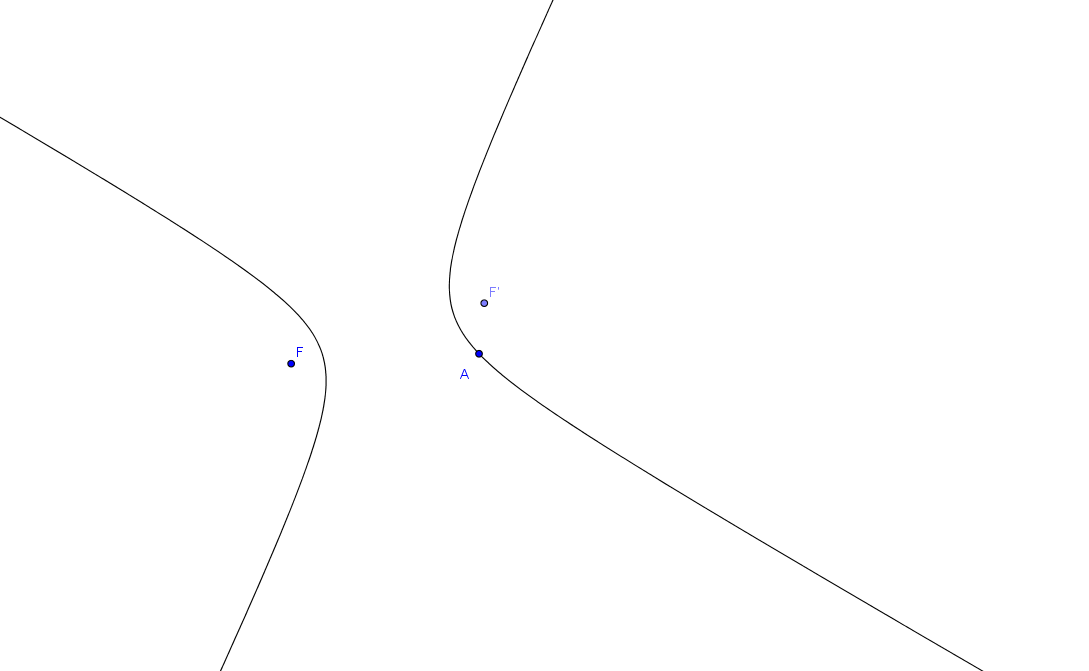
\includegraphics[width=\textwidth]{./hyperbole.png}
  \caption{Représentation d'une hyperbole}
  \label{fig:hyperbole}
\end{figure}


\section{Courbes définies par une équation cartésienne de degré deux}
\label{sec:eqcart}
\subsection{Problème}
On se donne six réels, $a$, $b$, $c$, $d$, $e$ et $f$ avec $a$, $b$, $c$ non tous nuls. On veut décrire la courbe $\con{{}}$ définie dans un repère orthonormal par l'équation cartésienne suivante~:
\begin{equation}
  ax^2+bxy+cy^2+dx+ey+f=0 \label{eq:con2gre2}
\end{equation}
Un paramètre important de~\eqref{eq:con2gre2} est son discriminant $\Delta=b^2-4ac$. L'idée est de reconnaître l'équation d'une conique par des changements de RON\@. On doit se débarrasser des termes $xy$ et de degré 1 en $x$ et $y$.

\subsection{Étape 1~: si $b\neq 0$, on se ramène par changement de repère à l'équation où $b=0$}
Soit $(\vect{u_{\varphi}},\vect{v_{\varphi}})$ la nouvelle BON\@. On va choisir $\varphi$ judicieusement pour que l'équation de la courbe $\con{{}}$ dans la nouvelle base n'ait pas de termes en $xy$. Si $M(x,y)$ dans $\rond$, on note $M(X,Y)$ ses coordonnées dans $(O,\vect{u}_\varphi,\vect{v}_\varphi)$ alors~:
$\begin{cases} x&=\cos\varphi X - \sin\varphi Y \\ y&=\sin\varphi X + \cos\varphi Y\end{cases}$ ainsi~:
\begin{align}
  ax^2&=a(\cos^2\varphi X^2 + \sin^2\varphi Y^2 - 2\cos\varphi\sin\varphi XY)\\
  bxy&=b(\cos\varphi X^2 -\sin\varphi\cos\varphi Y^2 + (\cos^2\varphi \sin^2\varphi)XY)\\
  cy^2&=c(\sin^2\varphi Y^2 + \cos^2\varphi X^2 + 2\cos\varphi\sin\varphi XY)
\end{align}
alors l'équation~\eqref{eq:con2gre2} est équivalente à~:
\begin{multline}
 (a\cos^2\varphi + b\cos\varphi\sin\varphi +c\sin^2\varphi)X^2+(a\sin^2\varphi - b\cos\varphi\sin\varphi +c\cos^2\varphi)Y^2\\+(2c\cos\varphi\sin\varphi-2a\cos\varphi\sin\varphi+b(\cos^2\varphi - \sin^2\varphi))XY + \\ (d\cos\varphi + e\sin\varphi)X +(e\cos\varphi - d\sin\varphi)Y +f=0
\end{multline}
c'est à dire qu'il existe six réels A,B,C,D,E et F tels que~:
\begin{equation}
  AX^2+BXY+CY^2+DX+EY+F=0 \label{eq:eqz}
\end{equation}
avec
\begin{equation}
 B=(c-a)\sin(2\varphi)+b\cos(2\varphi).
\end{equation}
Alors
\begin{equation}
 B=0 \iff \cotan(2\varphi)=\frac{a-c}{b}.
\end{equation}
Puisque la cotangente induit une bijection de $\intervalleoo{0}{\pi}$ sur $\R$ alors il existe un certain $\varphi$ tel que $B=0$. On choisit maintenant $\varphi$ tel que $B=0$. Montrons que $B^2-4AC=-4AC=b^2-4ac$~:
\begin{align}
  -4AC&=-4(a\cos^2\varphi+b\cos\varphi\sin\varphi +c\sin^2\varphi)(a\sin^2\varphi \\ &- b\cos\varphi\sin\varphi +c\cos^2\varphi) \notag\\
  &=-4(ac\cos^4\varphi + ac\sin^4\varphi+(a^2+c^2-b^2)\cos^2\varphi\sin^2\varphi\\ & +(bc-ab)\cos^3\varphi\sin\varphi+(ab-bc)\cos\varphi\sin^3\varphi) \notag\\
  &=-4(ac(\cos^2\varphi+\sin^2\varphi)^2+(a^2+c^2-b^2)\cos^2\sin^2\varphi \\ & +b(c-a)\cos\varphi\sin\varphi(\cos^2\varphi-\sin^2\varphi)) \notag\\
  &=-4ac-\sin^2(2\varphi)[(a-c)^2-b^2]-2b(c-a)\sin(2\varphi)\cos(2\varphi)
\end{align}
et puisque $B=0$, $\varphi$ vérifie $(c-a)\sin(2\varphi)=-b\cos(2\varphi)$, alors
\begin{align}
  -4AC&=-4ac-(a-c)^2\sin^2(2\varphi)+b^2\sin^2(2\varphi)+2b^2\cos^2(2\varphi)\\
  &=b^2-4ac-(a-c)^2\sin^2(2\varphi)+b^2\cos^2(2\varphi)\\
  &=b^2-4ac
\end{align}

\subsection{Étape 2~: disjonction des cas selon la valeur de $\Delta$}
\subsubsection{$\Delta=0$, la courbe $\con{{}}$ est du type parabole}
C'est à dire que $A=0$ ou $C=0$, quitte à faire un changement d'axe on suppose que $C=0$. Le réel $A$ est non nul sinon $(A,B,C)=(0,0,0)$. Alors~:
\begin{equation}
  AX^2+DX+EY+F=0 \iff A\left(X+\frac{D}{2A}\right)^2-\frac{AD^2}{4A^2}+EY+F=0
\end{equation}
on pose $\begin{cases}X'=X+\frac{D}{2A} \\ Y'=Y\end{cases}$ et $F'=F-\frac{D^2}{4A}$(on change d'origine) et on a~:
\begin{equation}
  AX'^2+EY'+F'=0.
\end{equation}
Plusieurs cas sont possibles~:
\begin{itemize}
\item si $E \neq 0$ alors $Y'=-\frac{A}{E}X'^2-\frac{F'}{E}$ et donc la courbe $\con{{}}$ est une parabole;
\item sinon alors $AX'^2+F'=0$
  \begin{itemize}
  \item si $\frac{F'}{A}>0$ alors $\con{{}}=\emptyset$;
  \item sinon si $F'=0$ alors $X'=0$ et $\con{{}}$ est une droite;
  \item sinon si $\frac{F'}{A}<0$ alors $X'=\pm \sqrt{\frac{-F'}{A}}$, et $\con{{}}$ est la réunion de deux droites parallèles.
  \end{itemize}
\end{itemize}

\subsubsection{$\Delta>0$, la courbe $\con{{}}$ est du type hyperbole}
Dans ce cas on a $AC<0$ et quitte à changer l'équation en son opposée, on peut supposer que $A>0$ et $C<0$. Alors l'équation~\eqref{eq:eqz} est équivalente à~:
\begin{equation}
  A\left(X+\frac{D}{2A}\right)^2 -A\frac{D^2}{4A^2} + C\left(Y+\frac{E}{2C}\right)^2 -C\frac{E^2}{4C^2}+F=0,
\end{equation}
puis en effectuant le changement de variable
\begin{equation}
  \begin{cases}
    X' = X+\frac{D}{2A} \\
    Y' = Y+\frac{E}{2C}
  \end{cases},
\end{equation}
alors on obtient (en posant $F'=F-\frac{D^2}{4A}-\frac{E^2}{4C}$):
\begin{equation}
  AX'^2+CY'^2+F'=0.
\end{equation}
Deux cas sont alors possibles~:
\begin{itemize}
\item si $F'=0$ alors $X'=\pm \sqrt{\frac{-C}{A}}$ et la courbe $\con{{}}$ est la réunion de deux droites sécantes d'équation $X'=\sqrt{\frac{-C}{A}}$ et $X'=-\sqrt{\frac{-C}{A}}$;
\item sinon alors $\frac{-C}{F'}Y^2-\frac{A}{F'}X^2=0$ et $\con{{}}$ est une hyperbole dont les asymptotes sont les droites précédentes.
\end{itemize}

\subsubsection{$\Delta<0$, la courbe $\con{{}}$ est du type ellipse}
Dans ce cas on a $AC<0$ et quitte à changer l'équation en son opposée, on peut supposer que $A>0$ et $C>0$. Alors l'équation~\eqref{eq:eqz} est équivalente à~:
\begin{equation}
  A\left(X+\frac{D}{2A}\right)^2 -A\frac{D^2}{4A^2} + C\left(Y+\frac{E}{2C}\right)^2 -C\frac{E^2}{4C^2}+F=0.
\end{equation}
En effectuant le changement de variable
\begin{equation}
  \begin{cases}
    X' = X+\frac{D}{2A}\\Y' = Y+\frac{E}{2C}
  \end{cases},
\end{equation}
on choisit une nouvelle origine $\Omega\left(-\frac{D}{2A},-\frac{E}{2C}\right)$. Alors on obtient (en posant $F'=F-\frac{D^2}{4A}-\frac{E^2}{4C}$)~:
\begin{equation}
  AX'^2+CY'^2+F'=0.
\end{equation}
Trois cas sont alors possibles~:
\begin{itemize}
\item si $F'>0$ alors $\con{{}}=\emptyset$;
\item si $F'=0$ alors $X'=Y'=0$ et donc $\con{{}}=\{\Omega\}$;
\item sinon $\frac{A}{-F'}X'^2+\frac{C}{-F'}Y'^2=1$ et~:
  \begin{itemize}
  \item si $A=C$ alors $\con{{}}$ est un cercle;
  \item sinon alors $\con{{}}$ est une ellipse.
  \end{itemize}
\end{itemize}
On parle de conique propre pour l'ellipse, l'hyperbole et la parabole; sinon on parle de conique dégénérée pour le cercle et les droites.

\section{Tangentes à une conique}
\subsection{Conique définie par une équation cartésienne}
Soient $a,b,c,d,e$ et $f$ six réels avec $a,b,c$ non tous nuls et $\con{{}}$ la conique d'équation~:
\begin{equation}
  ax^2+bxy+cy^2+dx+ey+f=0
\end{equation}
On suppose de plus que $\con{{}}$ est une conique propre. Nous avons vu dans la section~\ref{sec:eqred} que $\con{{}}$ peut être paramétrées par $(I,x,y)$ avec $x$ et $y$ dérivables. Nous rappelons que les équations étaient dans un bon repère telles que~:
\begin{itemize}
\item pour une parabole on a $\begin{cases} x(t) &= \frac{t^2}{2p} \\ y(t) &= t \end{cases}$;
\item pour une ellipse on a $\begin{cases} x(t) &= a\cos t\\ y(t) &= b\sin t \end{cases}$;
\item  et pour l'hyperbole $\begin{cases} x(t) &= \pm a\cosh t\\ y(t) &= \sinh t \end{cases}$.
\end{itemize}
On a aussi vu dans la section~\ref{sec:eqcart} que n'importe quelle conique admettait une équation cartésienne de degré deux telle que~:
\begin{equation}
\forall t \in I \quad   ax(t)^2+bx(t)y(t)+cy(t)^2+dx(t)+ey(t)+f=0
\end{equation}
Les fonctions $x$ et $y$ sont dérivables, alors si on dérive cette équation on a~:
\begin{equation}
  \forall t \in I \quad x'(t)+[2ax(t)+by(t)+d]+y'(t)+[2cy(t)+bx(t)+e]=0
\end{equation}
Montrons que si $(x_0,y_0)$ est un point de la courbe $\con{{}}$ alors $(2ax_0+by_0+d,2cy_0+bx_0+e)\neq (0,0)$.
\begin{proof}
  Soit $M_0(x_0,y_0)$ un point du plan qui vérifie le système suivant $\begin{cases}2ax_0+by_0+d &=0 \\ 2cy_0+bx_0+e &=0\end{cases}$. Si on pose les points $M(x,y)$ et $M'(2x_0-x,2y_0-y)$ alors après le développement des calculs on a~:
  \begin{align}
    a(2x_0-x)^2+b(2x_0-x)+c(2y_0-y)^2+d(2x_0-x)+e(2y_0-y)+f \notag \\
= ax(t)^2+bx(t)y(t)+cy(t)^2+dx(t)+ey(t)+f
  \end{align}
Alors $M \in \con{{}} \iff M' \in \con{{}}'$. Un tel point serait un centre de symétrie de $\con{{}}$. Deux cas sont possibles~:
\begin{itemize}
\item Si $\con{{}}$ est une parabole, un tel point n'existe pas;
\item sinon $M_0$ existe mais n'est pas sur $\con{{}}$.
\end{itemize}
En conclusion si un point $M_0(x_0,y_0)$ est sur $\con{{}}$ alors $2ax_0+by_0+d \neq 0$ ou $2cx_0+dy_0+e \neq 0$.
\end{proof}
Par conséquent, en un point $M_0(x_0,y_0)$ la conique $\con{{}}$ admet une tangente $T$ orthogonale à $\vect{u}=\begin{pmatrix} 2ax_0 +by_0 +d \\ 2cy_0+bx_0+e \end{pmatrix}$  alors~:
\begin{align}
M \in (T) &\iff \vect{M_0 M} \cdot \vect{u}=0 \\
&\iff (x-x_0)(2ax_0+by_0+d)+(y-y_0)(2cy_0+bx_0+e)=0 \\
&\iff 2axx_0 + b(xy_0+yx_0)+2cyy_0 +dx+ey - \alpha=0
\end{align}
avec
\begin{equation}
\alpha=2ax_0^2+  2bx_0y_0+2cy_0^2+dx_0+ey_0=-2f-dx_0-ey_0,
\end{equation}
puisque le point $M_0$ est sur la conique. Alors
\begin{equation}
  M \in (T) \iff 2axx_0+b(xy_0+x_0y)+2cyy_0+dx+e_y+dx_0+ey_0+2f=0.
\end{equation}
On dit que l'équation de la tangente $T$ à la courbe $\con{{}}$ est obtenue à partir de l'équation de $\con{{}}$ par la règle du dédoublement. En pratique $\frac{X^2}{a^2} + \frac{Y^2}{b^2}=1$ alors la tangente en un point $(x_0,y_0)$ est telle que
\begin{equation}
  \frac{1}{a^2}(2xx_0) + \frac{1}{b^2}(2yy_0)=2 \iff \frac{1}{a^2}(xx_0) + \frac{1}{b^2}(yy_0)=1.
\end{equation}

\subsection{Coniques définies par une équation polaire}

Soit $\con{{}}$ la conique d'équation polaire $\rho=\frac{p}{1+e\cos \theta}$ avec $e>0$ et $p=ed>0$. la fonction $\rho$ est dérivable. La tangente en un point $M_{\theta}$ de coordonnées polaires $(\rho(\theta),\theta)$ est dirigée par le vecteur $\rho'(\theta) \vect{u}_\theta + \rho(\theta) \vect{v}_\theta$ et on a~:
\begin{equation}
  \forall \theta \in \R \quad \rho'(\theta)=\frac{pe\sin\theta}{(1+e\cos\theta)^2},
\end{equation}
alors
\begin{equation}
  \rho'(\theta) \vect{u}_\theta + \rho(\theta) \vect{v}_\theta = \frac{p}{(1+e\cos\theta)^2} \vect{w}_\theta,
\end{equation}
avec $\vect{w}_\theta = e\sin\theta\vect{u}_\theta + (1+e\cos\theta)\vect{v}_\theta$ le vecteur directeur de la tangente $T$. Dans le repère $(O,\vect{u}_\theta, \vect{v}_\theta)$ soit $M(X,Y)$, alors
\begin{align}
  M \in T & \iff  \Det(\vect{M_\theta M},\vect{w}_\theta)=0 \\
  & \iff \begin{vmatrix} X-\rho(\theta) & e\sin\theta \\ Y & 1+e\cos\theta \end{vmatrix} = 0 \\
  & \iff X(1+e\cos\theta)-\rho(\theta)(1+e\cos\theta)-e\sin\theta Y = 0\\
  & \iff (1+e\cos\theta)X-e\sin\theta Y=p.
\end{align}
Si on note les coordonnées de $M(x,y)$ dans le repère initial $\rond$, alors
\begin{align}
  M \in T &\iff (1+e\cos\theta)(\cos\theta x+\sin\theta y)-e\sin\theta(-\sin\theta x+\cos\theta y)=p\\
&\iff (e+\cos\theta)x+\sin\theta y=p.
\end{align}

\subsection{Caractérisation géométrique des tangentes à une conique}
\subsubsection{Cas de la parabole}
\begin{prop}
  Soient $\P$ une parabole de foyer $F$ et de directrice $\Dr$, un point $M$ de $\P$ et son projeté orthogonal $H$ sur $\Dr$. Ainsi la tangente à $\P$ en M est la médiatrice du segment $[FH]$.
\end{prop}
\begin{proof}
  On se place dans le repère orthonormal direct $\rond$ dans lequel $\P$ a pour équation cartésienne $y^2=2px$, alors $F\left(\frac{p}{2},0\right)$ et $\Dr{}~: x=-\frac{p}{2}$. Soit $M_0(x_0,y_0)\in\P$, l'équation de la tangente à $\P$ en $M_0$ est $yy_0=p(x+x_0)$. Soit $I$ le point d'intersection de $T$ avec $(Oy)$ alors l'ordonnée du point I vaut $p\frac{x_0}{y_0}=\frac{y_0^2}{2y_0}=\frac{y_0}{2}$. Les coordonnées du point H sont $H\left(\frac{-p}{2}, y_0\right)$ et celle du foyer sont bien sûr $F\left(\frac{p}{2},0\right)$. Le point I est donc le milieu de $[HF]$ or $M_0\in\P$ donc $M_0H=M_0F$ donc $(M_0I)=T$ est la médiatrice de $[HF]$.
\end{proof}
\emph{Remarque}~: le point $M_0$ de la démonstration est confondu avec I si et seulement si $M_0=O$ et alors dans ce cas $T=(Oy)$ et c'est encore la médiatrice de $[HF]$.

\subsubsection{Cas de l'ellipse}
\begin{prop}
  Soit $\Ell$ une ellipse de foyer $F$ et $F'$. Soit $M$ un point de l'ellipse. La tangente $T$ en $M$ à l'ellipse est la bissectrice extérieure de l'angle $\widehat{F'MF}$.
\end{prop}
\begin{proof}
  Soient $(I,f(t))$ un paramétrage de l'ellipse avec $f$ une application dérivable et les applications $h=\norme{\vect{F'M}}$ $g=\norme{\vect{FM}}$. On sait que $g+h=2a$ avec $\vect{FM}$ et $\vect{F'M}$ tous deux non nuls (puisqu'on sait que les foyers ne sont pas sur l'ellipse). Alors $g$ et $h$ sont dérivables. Soit un réel $t$, alors~:
\begin{gather}
  g'(t)+h'(t)=0; \\
  \vect{FM}(t)=\vect{FO}+\vect{OM}(t), \quad \vect{F'M}(t)=\vect{F'O}+\vect{OM}(t);\\
  \derived{\vect{FM}}{t}=\derived{\vect{OM}}{t}, \quad \derived{\vect{F'M}}{t}=\derived{\vect{OM}}{t}.
\end{gather}
  Alors pour tout $t \in I$
  \begin{equation}
    0=g'(t)+h'(t)=\frac{\vect{FM}\cdot\derived{\vect{OM}}{t}}{\norme{\vect{FM}(t)}}\frac{\vect{F'M}\cdot\derived{\vect{OM}}{t}}{\norme{\vect{F'M}(t)}}=(\vect{u}+\vect{v})\cdot \derived{\vect{OM}}{t}.
  \end{equation}
Le vecteur $\derived{\vect{OM}}{t}$ est orthogonal au vecteur $(\vect{u}+\vect{v})$ avec $\vect{u}$ unitaire qui dirige $(FM)$ et $\vect{v}$ unitaire qui dirige $(F'M)$, donc $\vect{u}+\vect{v}$ dirige la bissectrice intérieure de $\widehat{F'MF}$. Alors $T$ est la droite passant par $M$ de vecteur normal $\vect{u}+\vect{v}$, donc $T$ est la bissectrice extérieure de l'angle $\widehat{F'MF}$.
\end{proof}

\subsubsection{Cas de l'hyperbole}
\begin{prop}
  Soient $\H$ une hyperbole de foyers $F$ et $F'$, $M$ un point de $\H$. La tangente $T$ à $\H$ en $M$ est la bissectrice intérieure de l'angle $\widehat{F'MF}$.
\end{prop}
\begin{proof}
  Soit $(I,f)$ un paramétrage d'une des deux branches de l'hyperbole avec $f$ dérivable. Soient les applications $h=\norme{\vect{F'M}}$ $g=\norme{\vect{FM}}$. On sait que pour tout point $M$ de l'hyperbole, $\abs{MF'-MF}=2a$. De plus, si on se place sur une des deux branche alors $MF'-MF$ est constant. Comme pour l'ellipse, les foyers n'appartiennent à l'hyperbole, donc $\vect{FM}(t)$ et $\vect{F'M}(t)$ sont toujours non nuls. Les fonction $g$ et $h$ sont ainsi dérivables sur $I$ et de manière analogue à l'ellipse on a~:
\begin{equation}
\forall t \in I \quad 0=g'(t)-h'(t)=(\vect{u}-\vect{v})\cdot \derived{\vect{OM}}{t}(t).
\end{equation}
 Le vecteur vitesse $\derived{\vect{OM}}{t}$ est orthogonal au vecteur $(\vect{u}-\vect{v})$ avec $\vect{u}$ unitaire qui dirige $(FM)$ et $\vect{v}$ unitaire qui dirige $(F'M)$, donc $\vect{u}-\vect{v}$ dirige la bissectrice extérieure de $\widehat{F'MF}$. Alors $T$ est la droite passant par $M$ de vecteur normal $\vect{u}-\vect{v}$, donc $T$ est la bissectrice intérieure de l'angle $\widehat{F'MF}$.
\end{proof}
